\documentclass[compress,aspectratio=169]{beamer}

\usepackage{lmodern}
\usepackage{ujslide}
\usepackage{graphicx}
\usepackage{url}
\usepackage[export]{adjustbox}
\usepackage{rotating}
\usepackage{booktabs}
\usepackage{amsmath}
\usepackage{multirow}
\usepackage{array}
\usepackage{tikz}
\usetikzlibrary{shapes.geometric, arrows.meta, positioning, fit, backgrounds}

\title{Detection of Suspicious Activities in Public Spaces Using Video Surveillance}
\subtitle{}
\author{Tshephang Phuti‑A‑Nkutu Matlala}
\institute[Academy of Computer Science and Software Engineering]{
  Academy of Computer Science and Software Engineering \\
  University of Johannesburg, Johannesburg, South Africa \\
  \url{223004635@student.uj.ac.za} \\
  \vspace{0.2cm}
  \footnotesize \textbf{Code:} \url{https://github.com/mat-tp/suspicious-activity-detection}
}
\date{\today}
\logo{
\includegraphics[height=15mm]{ujlogo.pdf}}

\newcommand{\standout}[1]{\begin{center}\LARGE\bfseries #1\end{center}}

\begin{document}

%----------------------------------------
%    TITLE SLIDE
%----------------------------------------
\begin{frame}
    \titlepage
\end{frame}

%----------------------------------------
%    OUTLINE SLIDE
%----------------------------------------
\section*{Outline}
\begin{frame}[allowframebreaks]{Outline}
    \tableofcontents
\end{frame}

% ===========================================================================
\section{Introduction}
% ===========================================================================

\begin{frame}{Motivation}
  \begin{itemize}
    \item Surveillance cameras are everywhere – train stations, malls, streets.
    \item Human operators cannot watch all feeds simultaneously; fatigue reduces attention.
    \item Need automatic activity recognition to \alert{assist} operators.
    \item Deep learning achieves high accuracy but requires:
      \begin{itemize}
        \item GPU hardware
        \item Huge labelled datasets (e.g., ActivityNet, YouTube-8M)
        \item Black‑box decisions – difficult to interpret in security contexts.
      \end{itemize}
  \end{itemize}
  \vfill
  \textbf{Goal:} A classical computer vision pipeline that is \alert{lightweight}, \alert{interpretable}, and \alert{robust} to poor video quality.
\end{frame}

\begin{frame}{Contributions}
  \begin{enumerate}
    \item Activity classification under \alert{authentic distortions} (focus, exposure, focus+exposure).
    \item First repurposing of the AD‑SVD dataset \emph{for classification} (originally designed for tracking).
    \item Head‑to‑head comparison of a \alert{from‑scratch Random Forest} with scikit‑learn's implementation.
    \item Dual‑mode evaluation: \alert{custom MOG2 detector} vs.\ dataset's ground‑truth bounding boxes to measure the impact of detection robustness.
  \end{enumerate}
\end{frame}

% ===========================================================================
\section{Dataset – AD‑SVD}
% ===========================================================================

\begin{frame}{AD‑SVD Dataset Overview}
  \begin{itemize}
    \item \textbf{4,476 videos}, 8 suspicious activities, 4 distortion types.
    \item Recorded indoors/outdoors, 7–10 FPS, fixed surveillance camera.
    \item \textbf{Activities:} Fighting in Group, Leaving Package, Passing Out, Person Pushing, Person Running, Prowl, Robbery with Knife, Walking.
    \item \textbf{Distortions:} Pristine (3.6\%), Exposure (32.3\%), Focus (31.5\%), Focus+Exposure (32.3\%).
    \item Ground‑truth bounding box for a single primary actor per frame.
    \item Publicly available: \alert{IEEE Dataport}.
  \end{itemize}
  \vspace{0.3cm}
  \footnotesize
  (Gomez‑Nieto et al., 2022; AD‑SVD)
\end{frame}

% Dataset Preview with YOUR images - Activity Classes
\begin{frame}{Dataset Preview – Activity Classes}
  \begin{columns}[T]
    \column{0.3\textwidth}
    \centering
    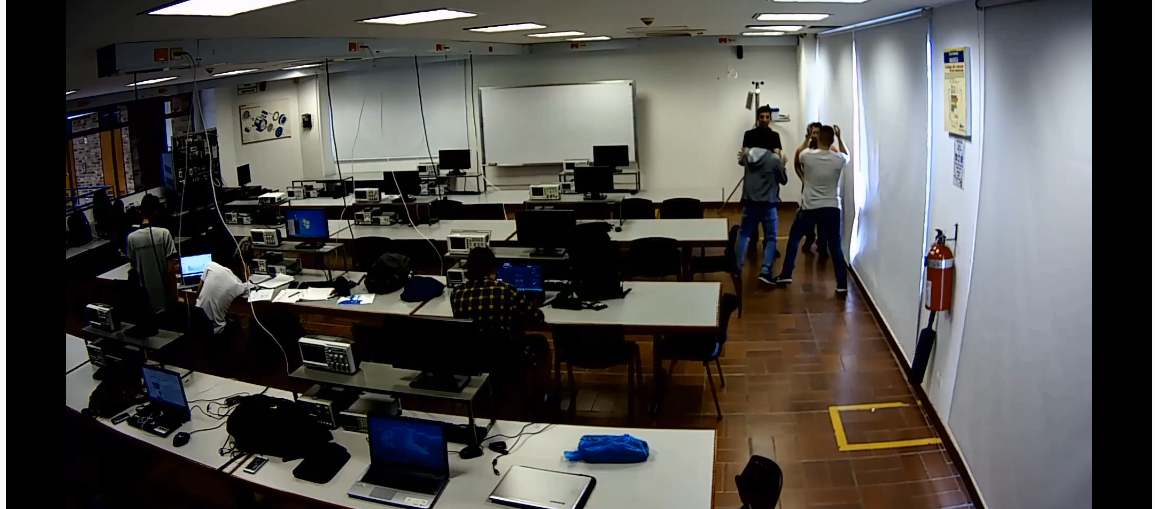
\includegraphics[width=\linewidth, height=2.5cm, keepaspectratio]{img/fighting.png}\\
    Fighting in Group
    
    \column{0.3\textwidth}
    \centering
    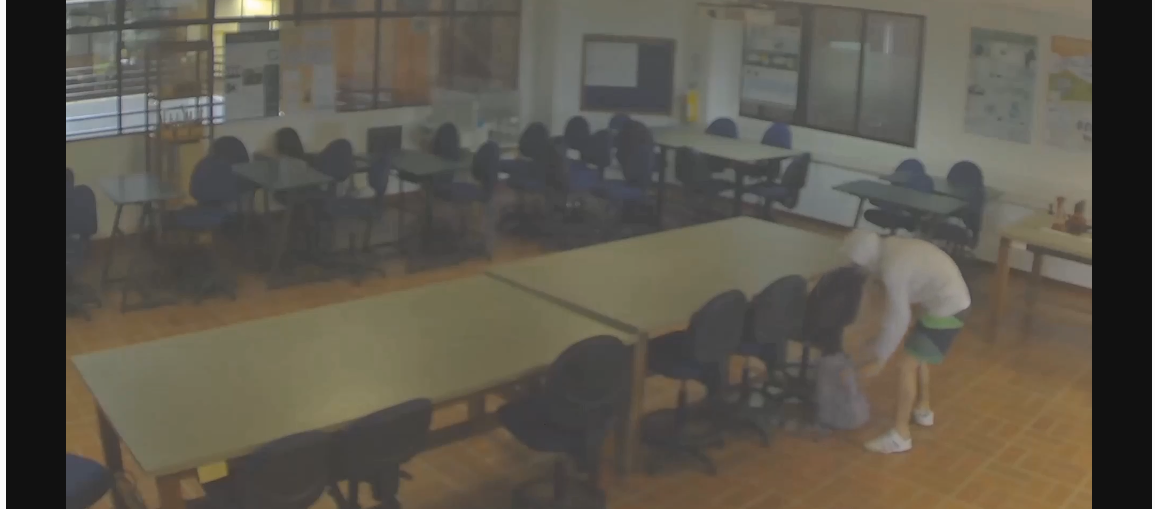
\includegraphics[width=\linewidth, height=2.5cm, keepaspectratio]{img/leaving_package.png}\\
    Leaving Package
    
    \column{0.3\textwidth}
    \centering
    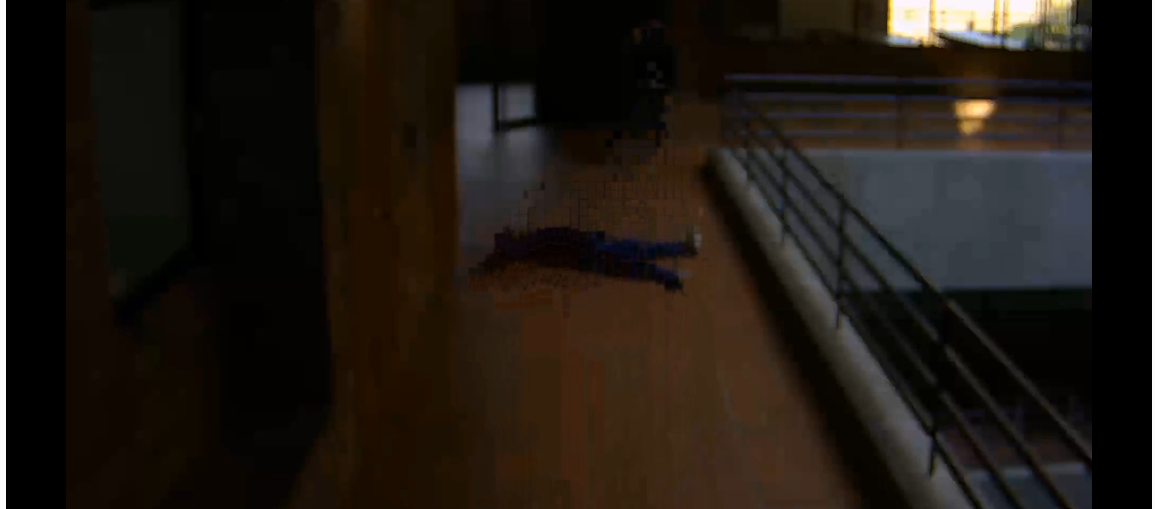
\includegraphics[width=\linewidth, height=2.5cm, keepaspectratio]{img/passing_out.png}\\
    Passing Out
  \end{columns}
  
  \vspace{0.3cm}
  
  \begin{columns}[T]
    \column{0.3\textwidth}
    \centering
    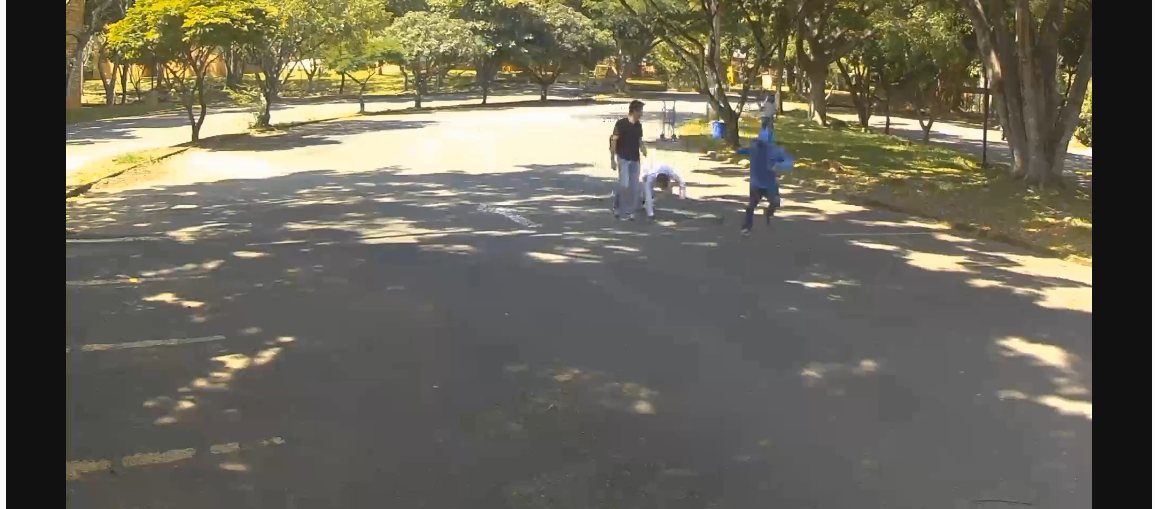
\includegraphics[width=\linewidth, height=2.5cm, keepaspectratio]{img/pushing.png}\\
    Person Pushing
    
    \column{0.3\textwidth}
    \centering
    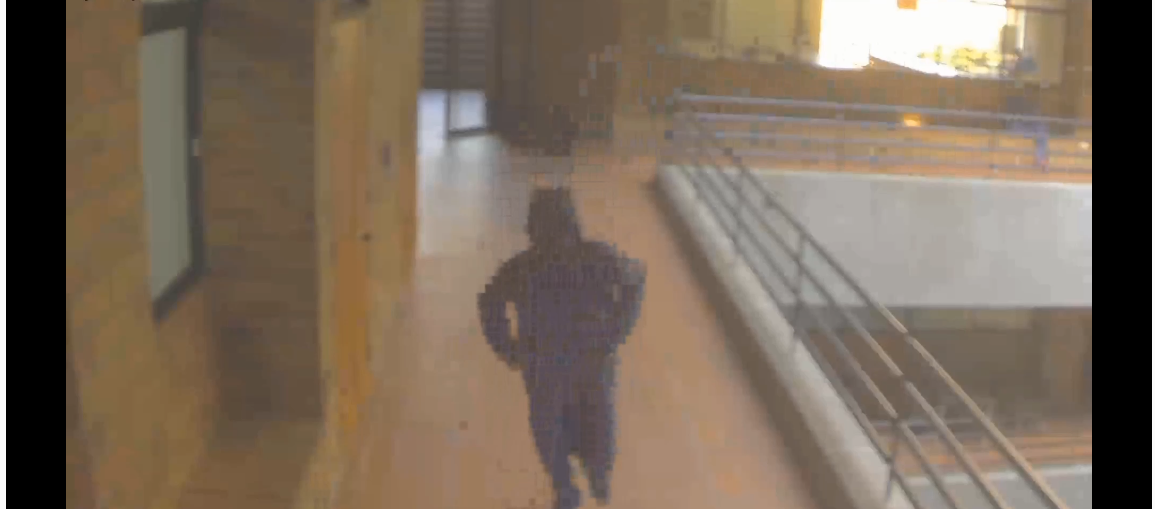
\includegraphics[width=\linewidth, height=2.5cm, keepaspectratio]{img/running.png}\\
    Person Running
    
    \column{0.3\textwidth}
    \centering
    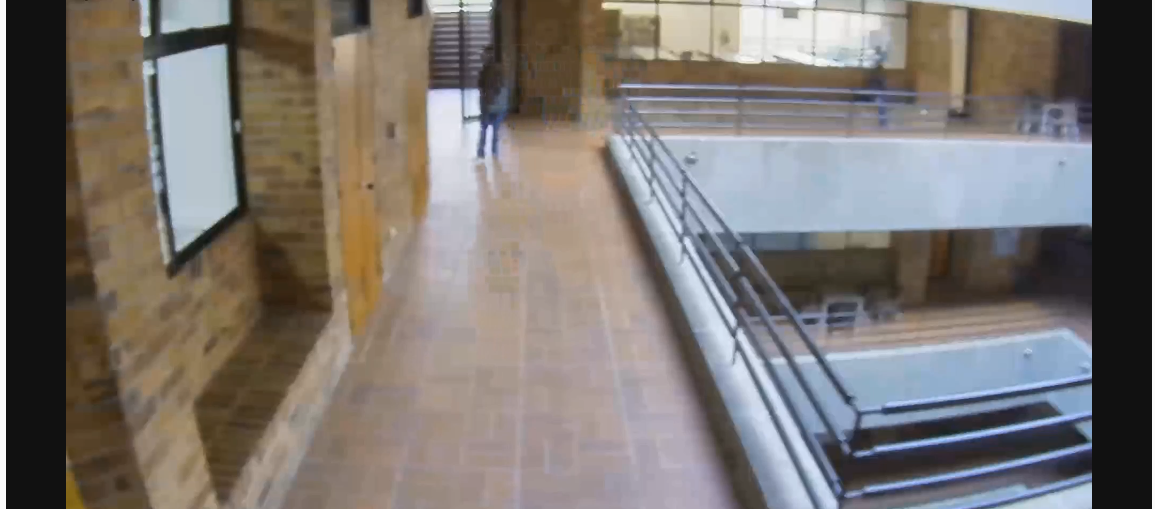
\includegraphics[width=\linewidth, height=2.5cm, keepaspectratio]{img/prowl.png}\\
    Prowl
  \end{columns}
  
  \vspace{0.3cm}
  
  \begin{columns}[T]
    \column{0.3\textwidth}
    \centering
    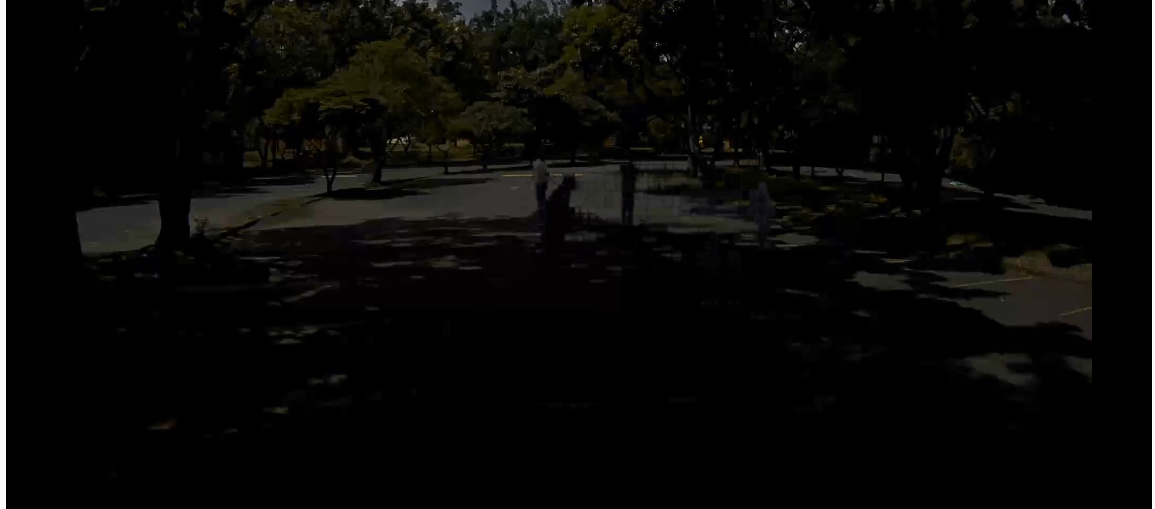
\includegraphics[width=\linewidth, height=2.5cm, keepaspectratio]{img/robbery.png}\\
    Robbery with Knife
    
    \column{0.3\textwidth}
    \centering
    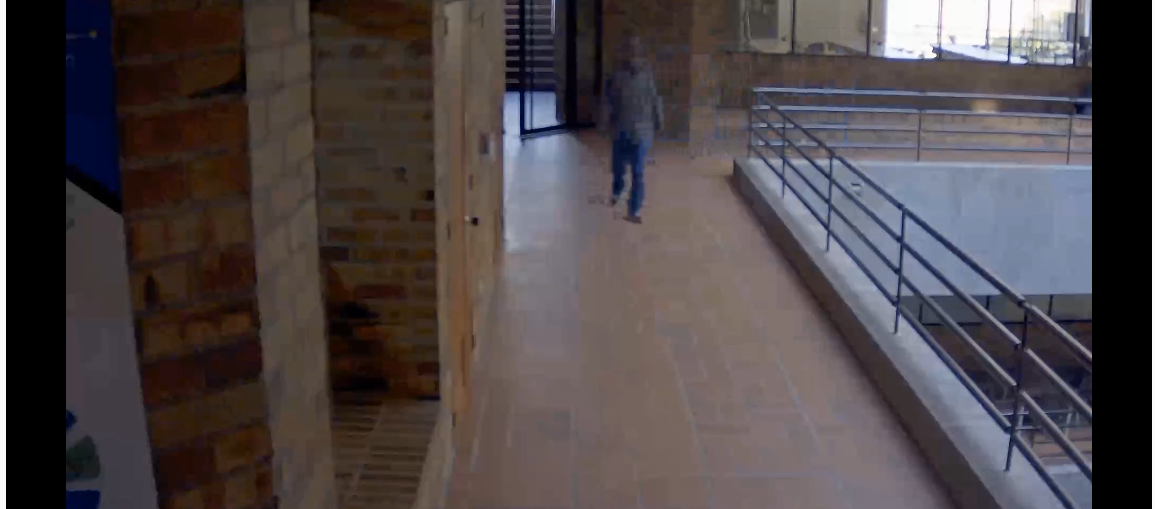
\includegraphics[width=\linewidth, height=2.5cm, keepaspectratio]{img/walking.png}\\
    Walking
    
    \column{0.3\textwidth}
    \centering
    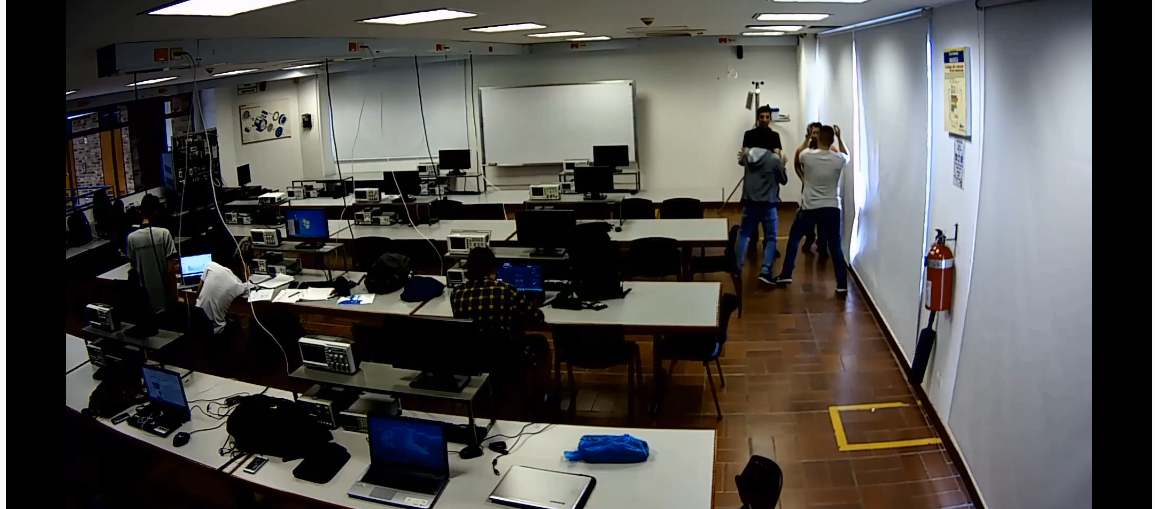
\includegraphics[width=\linewidth, height=2.5cm, keepaspectratio]{img/fighting.png}\\
    (More samples)
  \end{columns}
\end{frame}

% Dataset Preview - Distortion Types
\begin{frame}{Dataset Preview – Distortion Types}
  \begin{columns}[T]
    \column{0.23\textwidth}
    \centering
    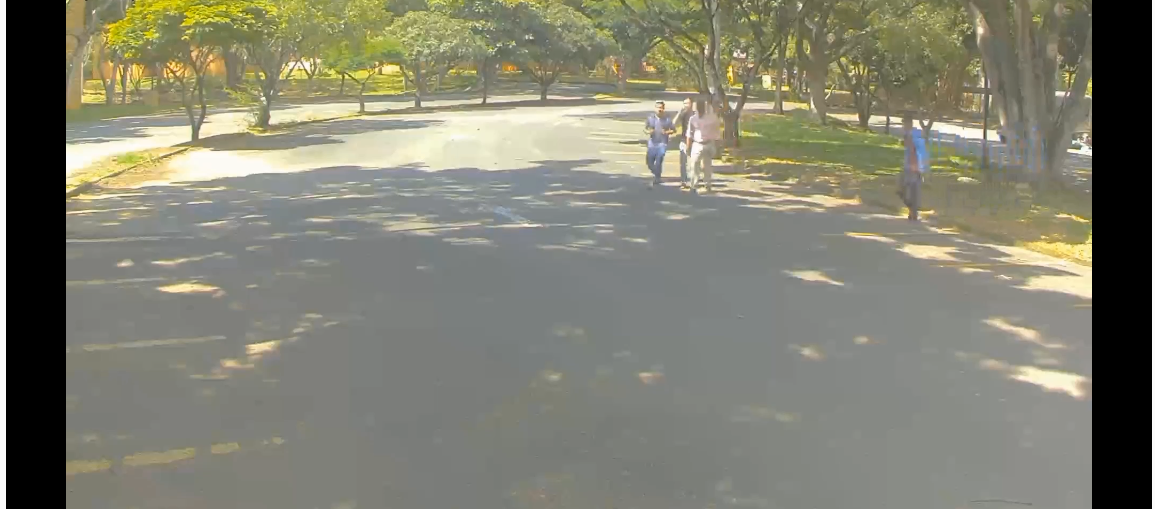
\includegraphics[width=\linewidth, height=2.5cm, keepaspectratio]{img/pristine.jpg}\\
    \textbf{Pristine}
    
    \column{0.23\textwidth}
    \centering
    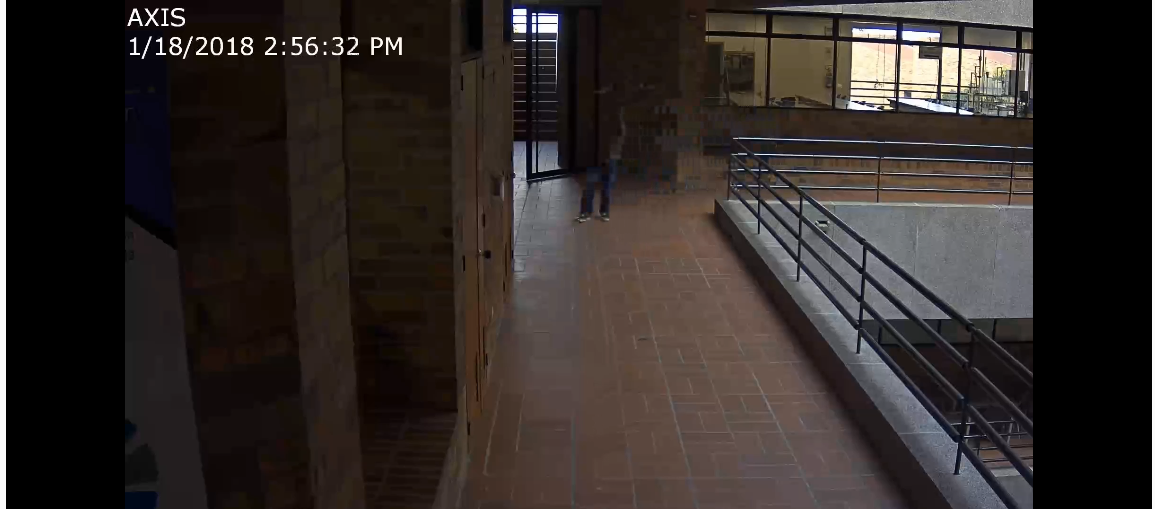
\includegraphics[width=\linewidth, height=2.5cm, keepaspectratio]{img/exposure.jpg}\\
    \textbf{Exposure}
    
    \column{0.23\textwidth}
    \centering
    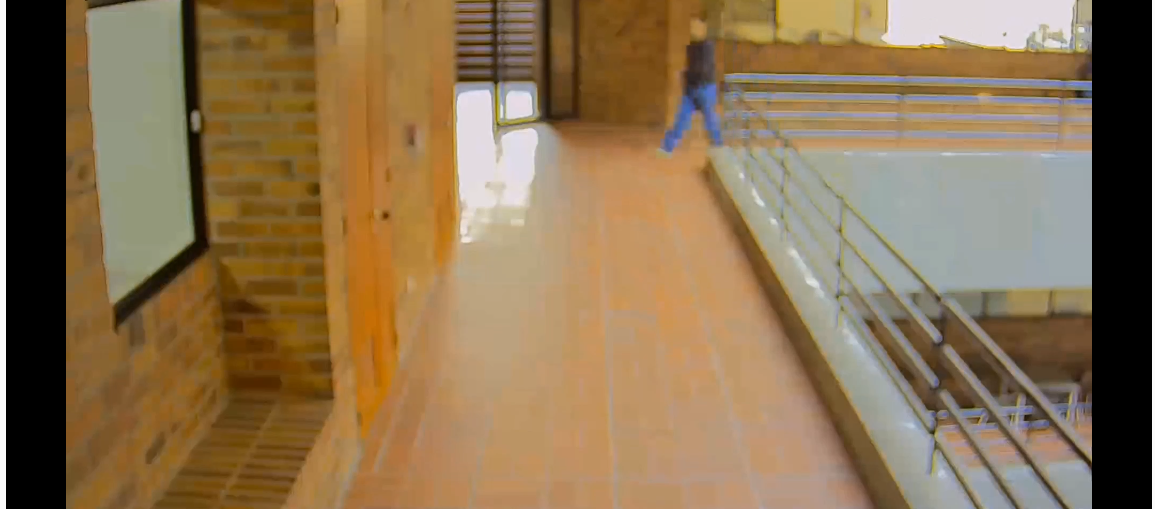
\includegraphics[width=\linewidth, height=2.5cm, keepaspectratio]{img/focus.jpg}\\
    \textbf{Focus}
    
    \column{0.23\textwidth}
    \centering
    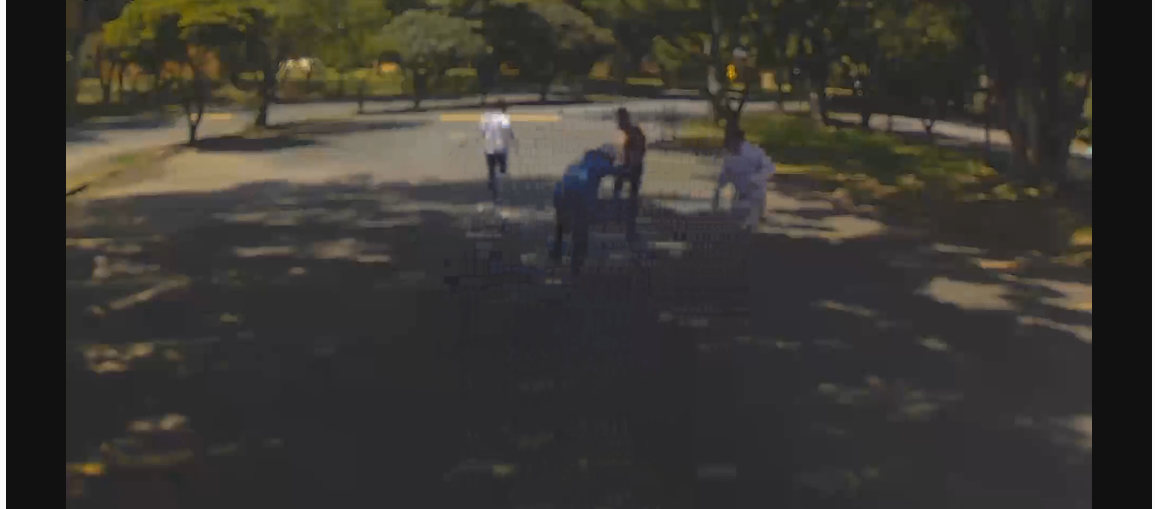
\includegraphics[width=\linewidth, height=2.5cm, keepaspectratio]{img/exfo.jpg}\\
    \textbf{Focus+Exposure}
  \end{columns}
  
  \vspace{0.5cm}
  \begin{itemize}
    \item \textbf{Focus blur} diffuses object boundaries → detection often fails.
    \item \textbf{Exposure changes} reduce foreground‑background contrast.
    \item Almost \textbf{96\%} of videos are distorted — testing ground for robustness.
  \end{itemize}
\end{frame}

\begin{frame}{Challenge: Distortion Effects}
  \centering
  \small
  \begin{tabular}{lrr}
    \toprule
    Distortion Type & Videos & \% of total \\
    \midrule
    Focus and Exposure (ExFo) & 1,447 & 32.3\% \\
    Exposure (Exp)            & 1,445 & 32.3\% \\
    Focus (Fo)                & 1,409 & 31.5\% \\
    Pristine (Pri)            &   160 &  3.6\% \\
    \bottomrule
  \end{tabular}
  \vspace{0.5cm}
  
  \centering
  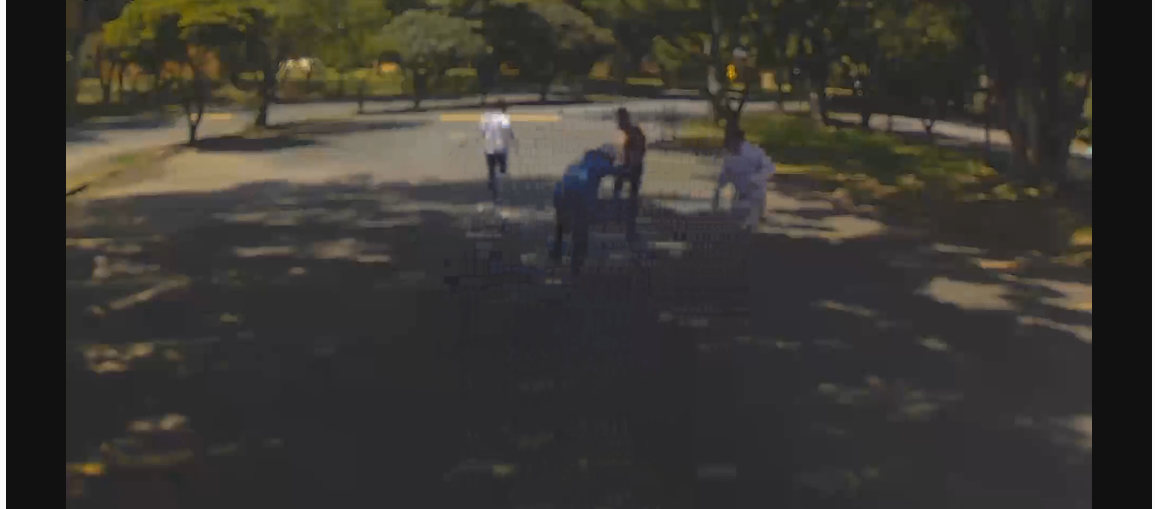
\includegraphics[width=0.6\textwidth]{img/exfo.jpg}
  
  \medskip
  \footnotesize Example of severe Focus+Exposure distortion
\end{frame}

% ===========================================================================
\section{Method}
% ===========================================================================

\begin{frame}{Pipeline Overview}
  \begin{center}
    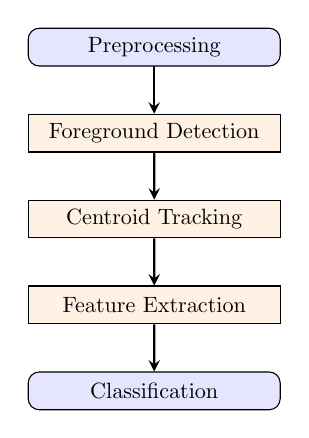
\begin{tikzpicture}[node distance=0.6cm, scale=0.8, every node/.style={scale=0.8}]
      \node (pre) [rectangle, rounded corners, minimum width=4cm, minimum height=0.6cm, align=center, draw=black, fill=blue!10] {Preprocessing};
      \node (fg)  [rectangle, minimum width=4cm, minimum height=0.6cm, align=center, draw=black, fill=orange!10, below=of pre] {Foreground Detection};
      \node (track) [rectangle, minimum width=4cm, minimum height=0.6cm, align=center, draw=black, fill=orange!10, below=of fg] {Centroid Tracking};
      \node (feat) [rectangle, minimum width=4cm, minimum height=0.6cm, align=center, draw=black, fill=orange!10, below=of track] {Feature Extraction};
      \node (class) [rectangle, rounded corners, minimum width=4cm, minimum height=0.6cm, align=center, draw=black, fill=blue!10, below=of feat] {Classification};
      \draw [->, >=stealth, thick] (pre) -- (fg);
      \draw [->, >=stealth, thick] (fg) -- (track);
      \draw [->, >=stealth, thick] (track) -- (feat);
      \draw [->, >=stealth, thick] (feat) -- (class);
    \end{tikzpicture}
  \end{center}
  \vspace{0.3cm}
  \footnotesize
  \textbf{Stages:} Pre-processing $\rightarrow$ Foreground Detection $\rightarrow$ Centroid Tracking $\rightarrow$ Optical Flow $\rightarrow$ Feature Extraction $\rightarrow$ Classifier.
\end{frame}

\begin{frame}{Detection Modes}
  \begin{columns}[t]
    \column{0.48\textwidth}
    \textbf{MOG2 (our detector)}
    \begin{itemize}
      \item Gaussian Mixture Model background subtraction.
      \item Morphological cleaning, blob size filtering ($>500$ px$^2$).
      \item Can produce \emph{multiple} detections per frame.
      \item \alert{Fails on most Focus \& ExFo videos} (blur hides foreground).
    \end{itemize}
    \column{0.48\textwidth}
    \textbf{Ground‑truth (GT) boxes}
    \begin{itemize}
      \item One bounding box per frame, from human annotation.
      \item Exactly \emph{one} track per video.
      \item Unaffected by distortion.
      \item Used to study the \alert{upper bound} of classification performance.
    \end{itemize}
  \end{columns}
  \vspace{0.3cm}
  \small
  \textbf{MOG2} yields only 848 usable videos (19\%)\hspace{0.5cm}\textbf{GT} yields 4,461 videos (99.7\%).
\end{frame}

\begin{frame}{Tracking \& Feature Extraction}
  \textbf{Centroid Tracking}
  \begin{itemize}
    \item Greedy nearest‑neighbour match using Euclidean distance.
    \item Tracks shorter than 30 frames are discarded → removes spurious background blobs.
  \end{itemize}
  \vspace{0.1cm}
  \textbf{14 Per‑track Features}
  \begin{itemize}
    \item Trajectory geometry: length, total distance, net displacement, straightness, area.
    \item Speed statistics: mean, max, std, skewness, kurtosis.
    \item Direction statistics: mean and std of heading angle.
    \item Global optical flow: mean magnitude \& angle (Lucas‑Kanade).
  \end{itemize}
  \vspace{0.1cm}
  \textbf{Per‑video aggregation:} mean, max, std of each per‑track feature + number of tracks → \alert{43 features per video}.
\end{frame}

\begin{frame}{Random Forest: A Quick Overview}
  \centering
  \small
  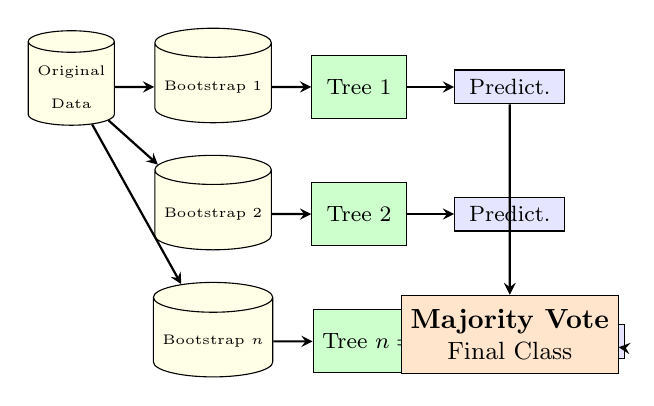
\begin{tikzpicture}[
    node distance=0.5cm,
    tree/.style={rectangle, draw=black, fill=green!10, minimum width=1.2cm, minimum height=0.8cm, align=center},
    data/.style={draw, cylinder, shape border rotate=90, aspect=0.25, fill=yellow!10, minimum height=1.2cm, align=center},
    arrow/.style={->, >=stealth, thick},
  ]
  
  % Bootstrap samples
  \node[data] (orig) {\tiny Original\\ \tiny Data};
  \node[data, right=0.5cm of orig] (boot1) {\tiny Bootstrap 1};
  \node[data, below=0.4cm of boot1] (boot2) {\tiny Bootstrap 2};
  \node[data, below=0.4cm of boot2] (bootn) {\tiny Bootstrap $n$};
  
  \draw[arrow] (orig) -- (boot1);
  \draw[arrow] (orig) -- (boot2);
  \draw[arrow] (orig) -- (bootn);
  
  % Trees
  \node[tree, right=0.5cm of boot1, fill=green!20] (t1) {\footnotesize Tree 1};
  \node[tree, right=0.5cm of boot2, fill=green!20] (t2) {\footnotesize Tree 2};
  \node[tree, right=0.5cm of bootn, fill=green!20] (tn) {\footnotesize Tree $n=200$};
  
  \draw[arrow] (boot1) -- (t1);
  \draw[arrow] (boot2) -- (t2);
  \draw[arrow] (bootn) -- (tn);
  
  % Predictions
  \node[rectangle, draw=black, fill=blue!10, minimum width=1.4cm, right=0.6cm of t1] (p1) {\footnotesize Predict.};
  \node[rectangle, draw=black, fill=blue!10, minimum width=1.4cm, right=0.6cm of t2] (p2) {\footnotesize Predict.};
  \node[rectangle, draw=black, fill=blue!10, minimum width=1.4cm, right=0.6cm of tn] (pn) {\footnotesize Predict.};
  
  \draw[arrow] (t1) -- (p1);
  \draw[arrow] (t2) -- (p2);
  \draw[arrow] (tn) -- (pn);
  
    % Majority vote
  \node[rectangle, draw=black, fill=orange!20, minimum width=2.5cm, minimum height=1cm,
        align=center, below=0.8cm of p2] (vote) {\textbf{Majority Vote}\\[-0.1em]\small Final Class};
  \draw[arrow] (p1) -- (vote);
  \draw[arrow] (p2) -- (vote);
  \draw[arrow] (pn) -- (vote);
  
  \end{tikzpicture}
  
  \vspace{0.3cm}
  \begin{columns}[t]
    \column{0.48\textwidth}
    \textbf{How it works}
    \begin{itemize}
      \item Ensemble of many decision trees.
      \item Each tree trained on a \alert{bootstrap sample} (bagging).
      \item At each split, a \alert{random subset} of $\sqrt{d}$ features is considered.
      \item Trees vote; majority wins.
    \end{itemize}
    \column{0.48\textwidth}
    \textbf{Why we use it}
    \begin{itemize}
      \item Resists overfitting, handles small sample sizes.
      \item Works well with our 43‑D hand‑crafted features.
      \item Provides \alert{feature importance} for interpretability.
      \item We compare a \alert{custom implementation} (200 trees, depth=10) with scikit‑learn's.
    \end{itemize}
  \end{columns}
\end{frame}

\begin{frame}{Classifiers}
  Four models evaluated on the same 43‑dimensional features:
  \begin{itemize}
    \item \textbf{SVM} (RBF kernel, $C=10$, balanced class weights).
    \item \textbf{K‑Nearest Neighbours} ($k=10$).
    \item \textbf{Random Forest} – scikit‑learn (200 trees, balanced weights, unconstrained depth).
    \item \textbf{Custom Random Forest} – built from scratch (200 trees, max depth 10, entropy split, bootstrap, $\sqrt{d}$ features per split).
  \end{itemize}
  \vspace{0.3cm}
  \small
  Data split: 70\% train, 15\% validation, 15\% test (stratified).\\
  Features standardised inside a pipeline.
\end{frame}

% ===========================================================================
\section{Results}
% ===========================================================================

\begin{frame}{Activity Classification – GT Mode (4,461 videos)}
  \begin{columns}
    \column{0.55\textwidth}
    \small
    \begin{tabular}{lrr}
      \toprule
      Classifier & Test Acc. & CV Mean \\
      \midrule
      SVM (RBF)      & 76.4\% & 73.7\% \\
      KNN ($k=10$)   & 69.6\% & 68.5\% \\
      \alert{RF (sklearn)} & \alert{94.0\%} & 91.1\% \\
      Custom RF      & 92.5\% (val) & --- \\
      \midrule
      Random (8-cl.) & 12.5\% & --- \\
      \bottomrule
    \end{tabular}

    \column{0.45\textwidth}
    \small
    \textbf{Top per‑class F1:}
    \begin{itemize}
      \item Person Running: \textbf{0.99}
      \item Passing Out: 0.96
      \item Prowl: 0.96
      \item Fighting: 0.95
      \item Walking: 0.95
    \end{itemize}
    \vspace{0.2cm}
    \alert{Macro avg F1 = 0.94}
  \end{columns}
\end{frame}

% Confusion Matrix
\begin{frame}{Confusion Matrix – GT Mode (sklearn RF)}
  \centering
  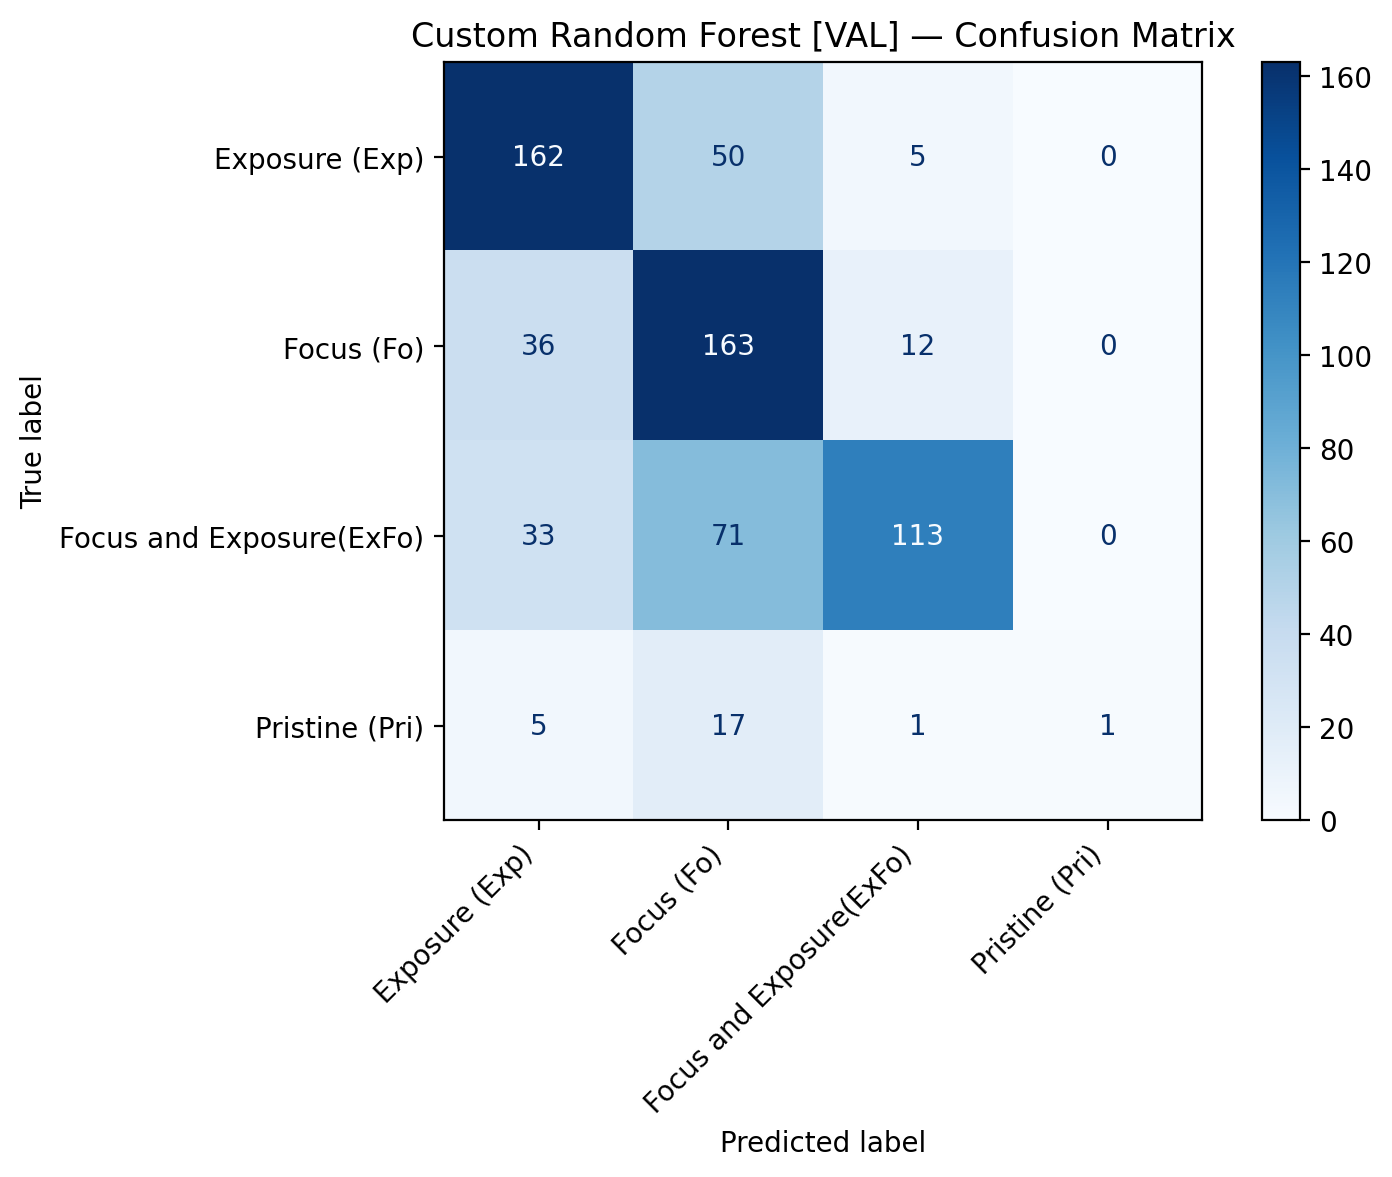
\includegraphics[width=0.8\textwidth]{img/confusion_matrix.png}
  
  \medskip
  \footnotesize Normalised confusion matrix of 8 activity classes.
\end{frame}

% Feature Importance
\begin{frame}{Feature Importance (Random Forest)}
  \centering
  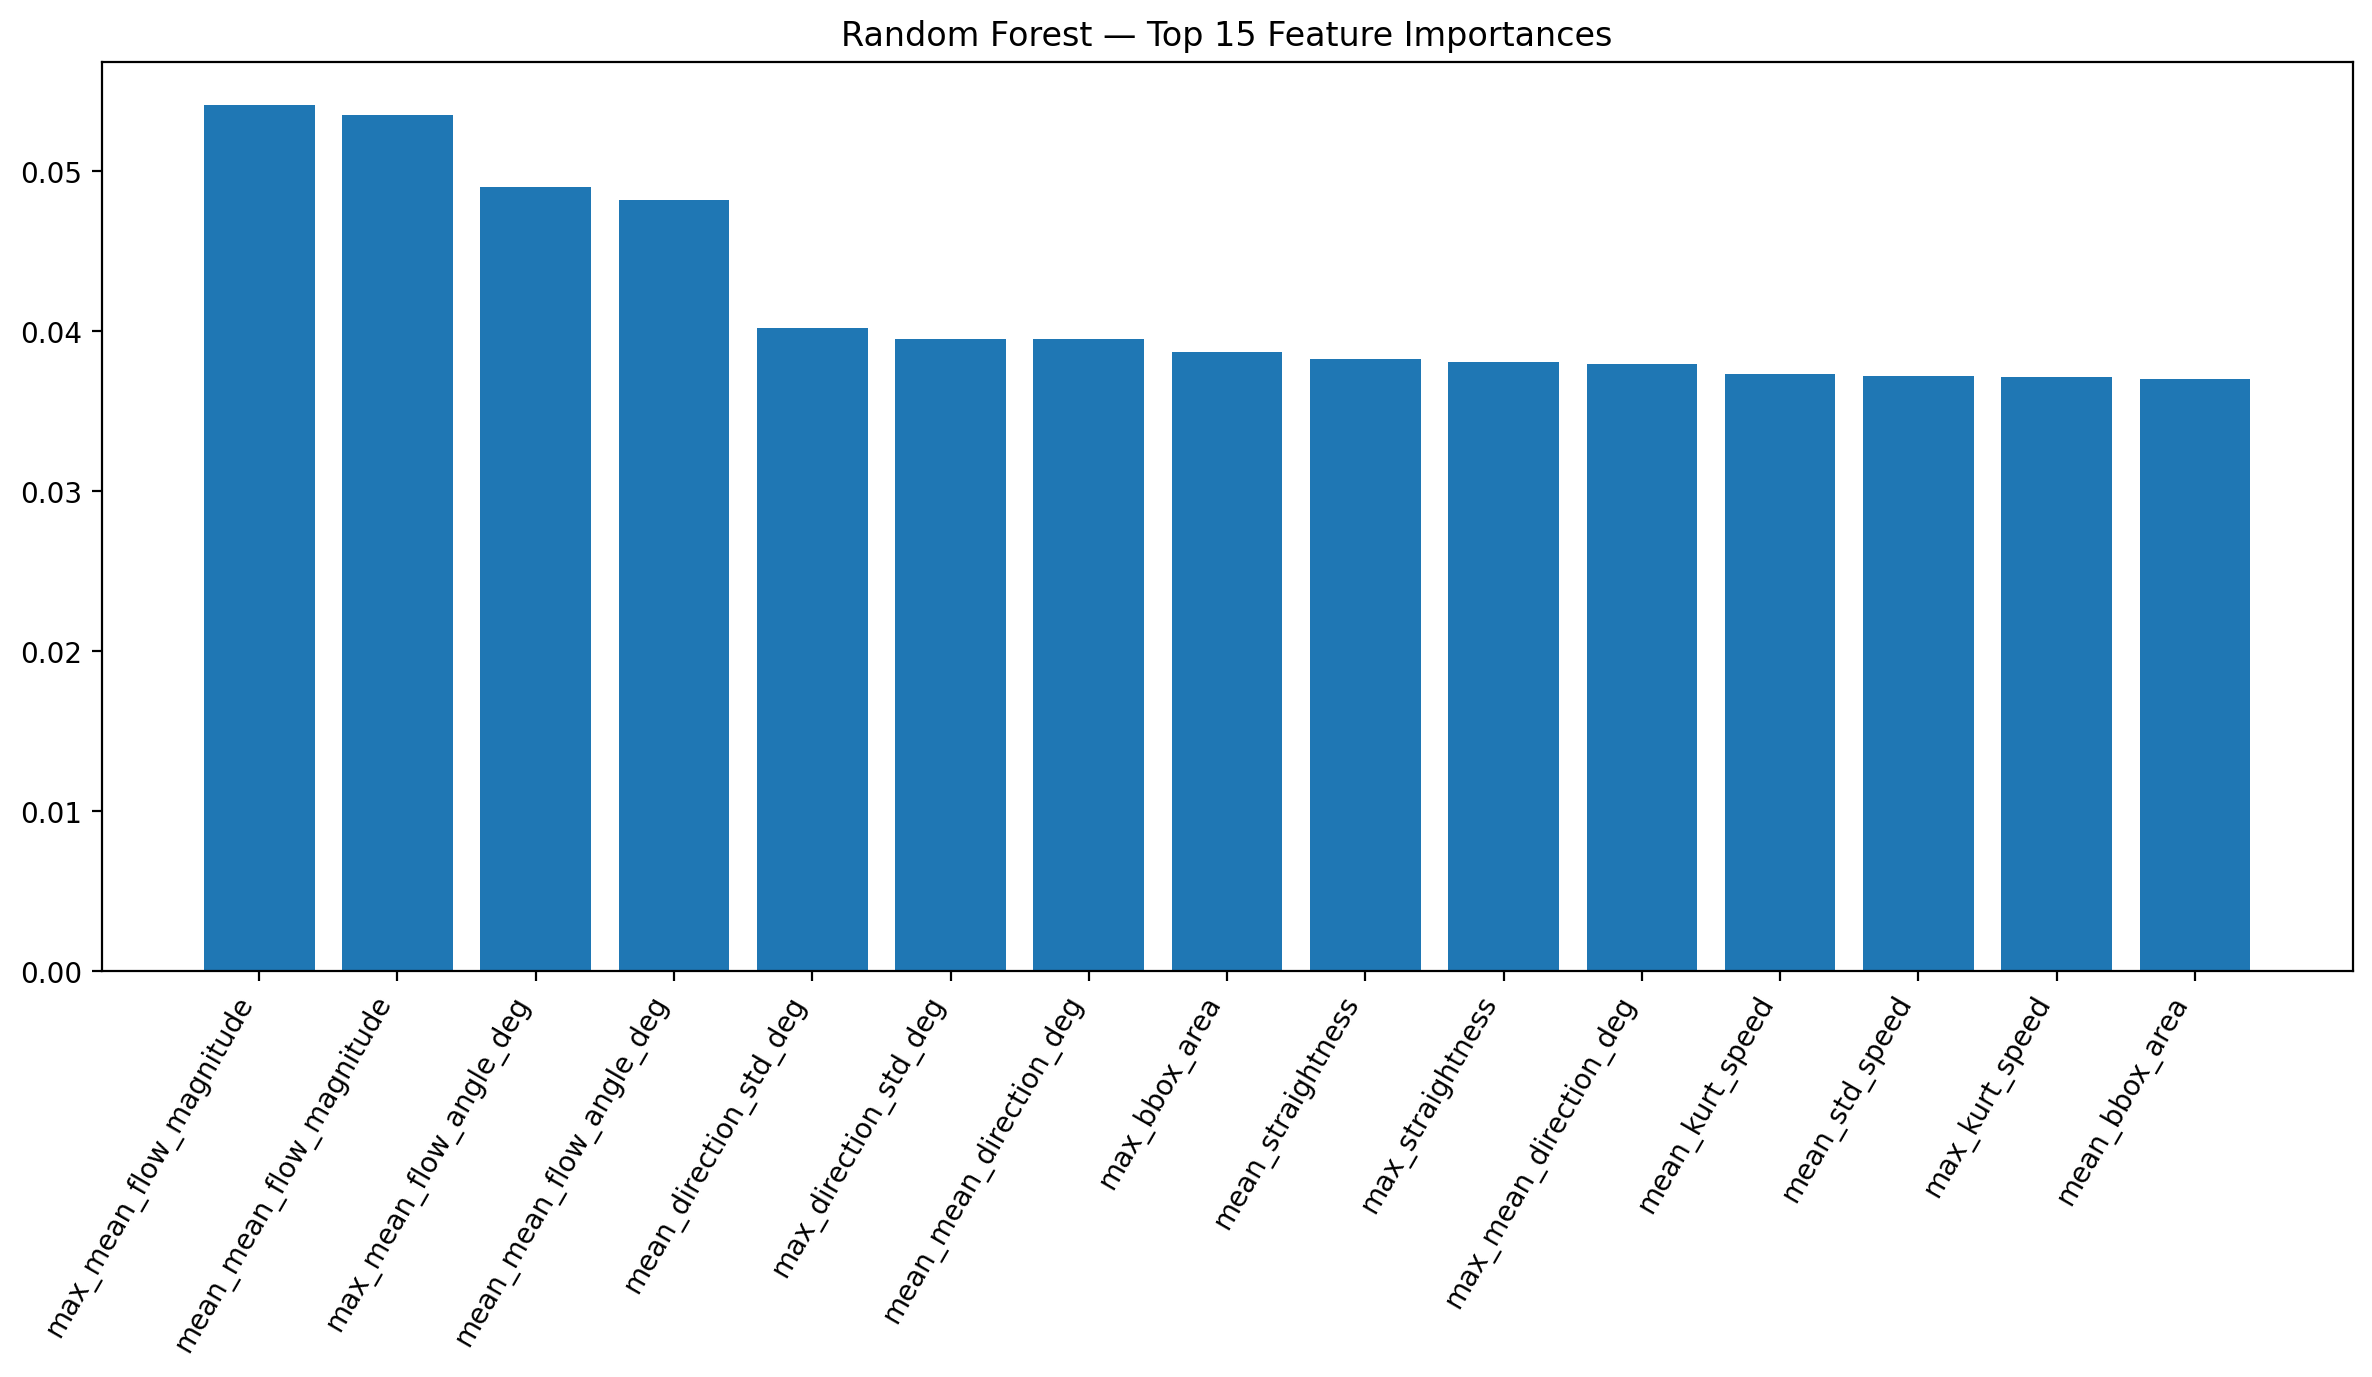
\includegraphics[width=0.8\textwidth]{img/feature_importance.png}
  
  \medskip
  \footnotesize Top features from the sklearn Random Forest (GT mode).
\end{frame}

% Accuracy Comparison
\begin{frame}{Accuracy Comparison – Activity Classification}
  \centering
  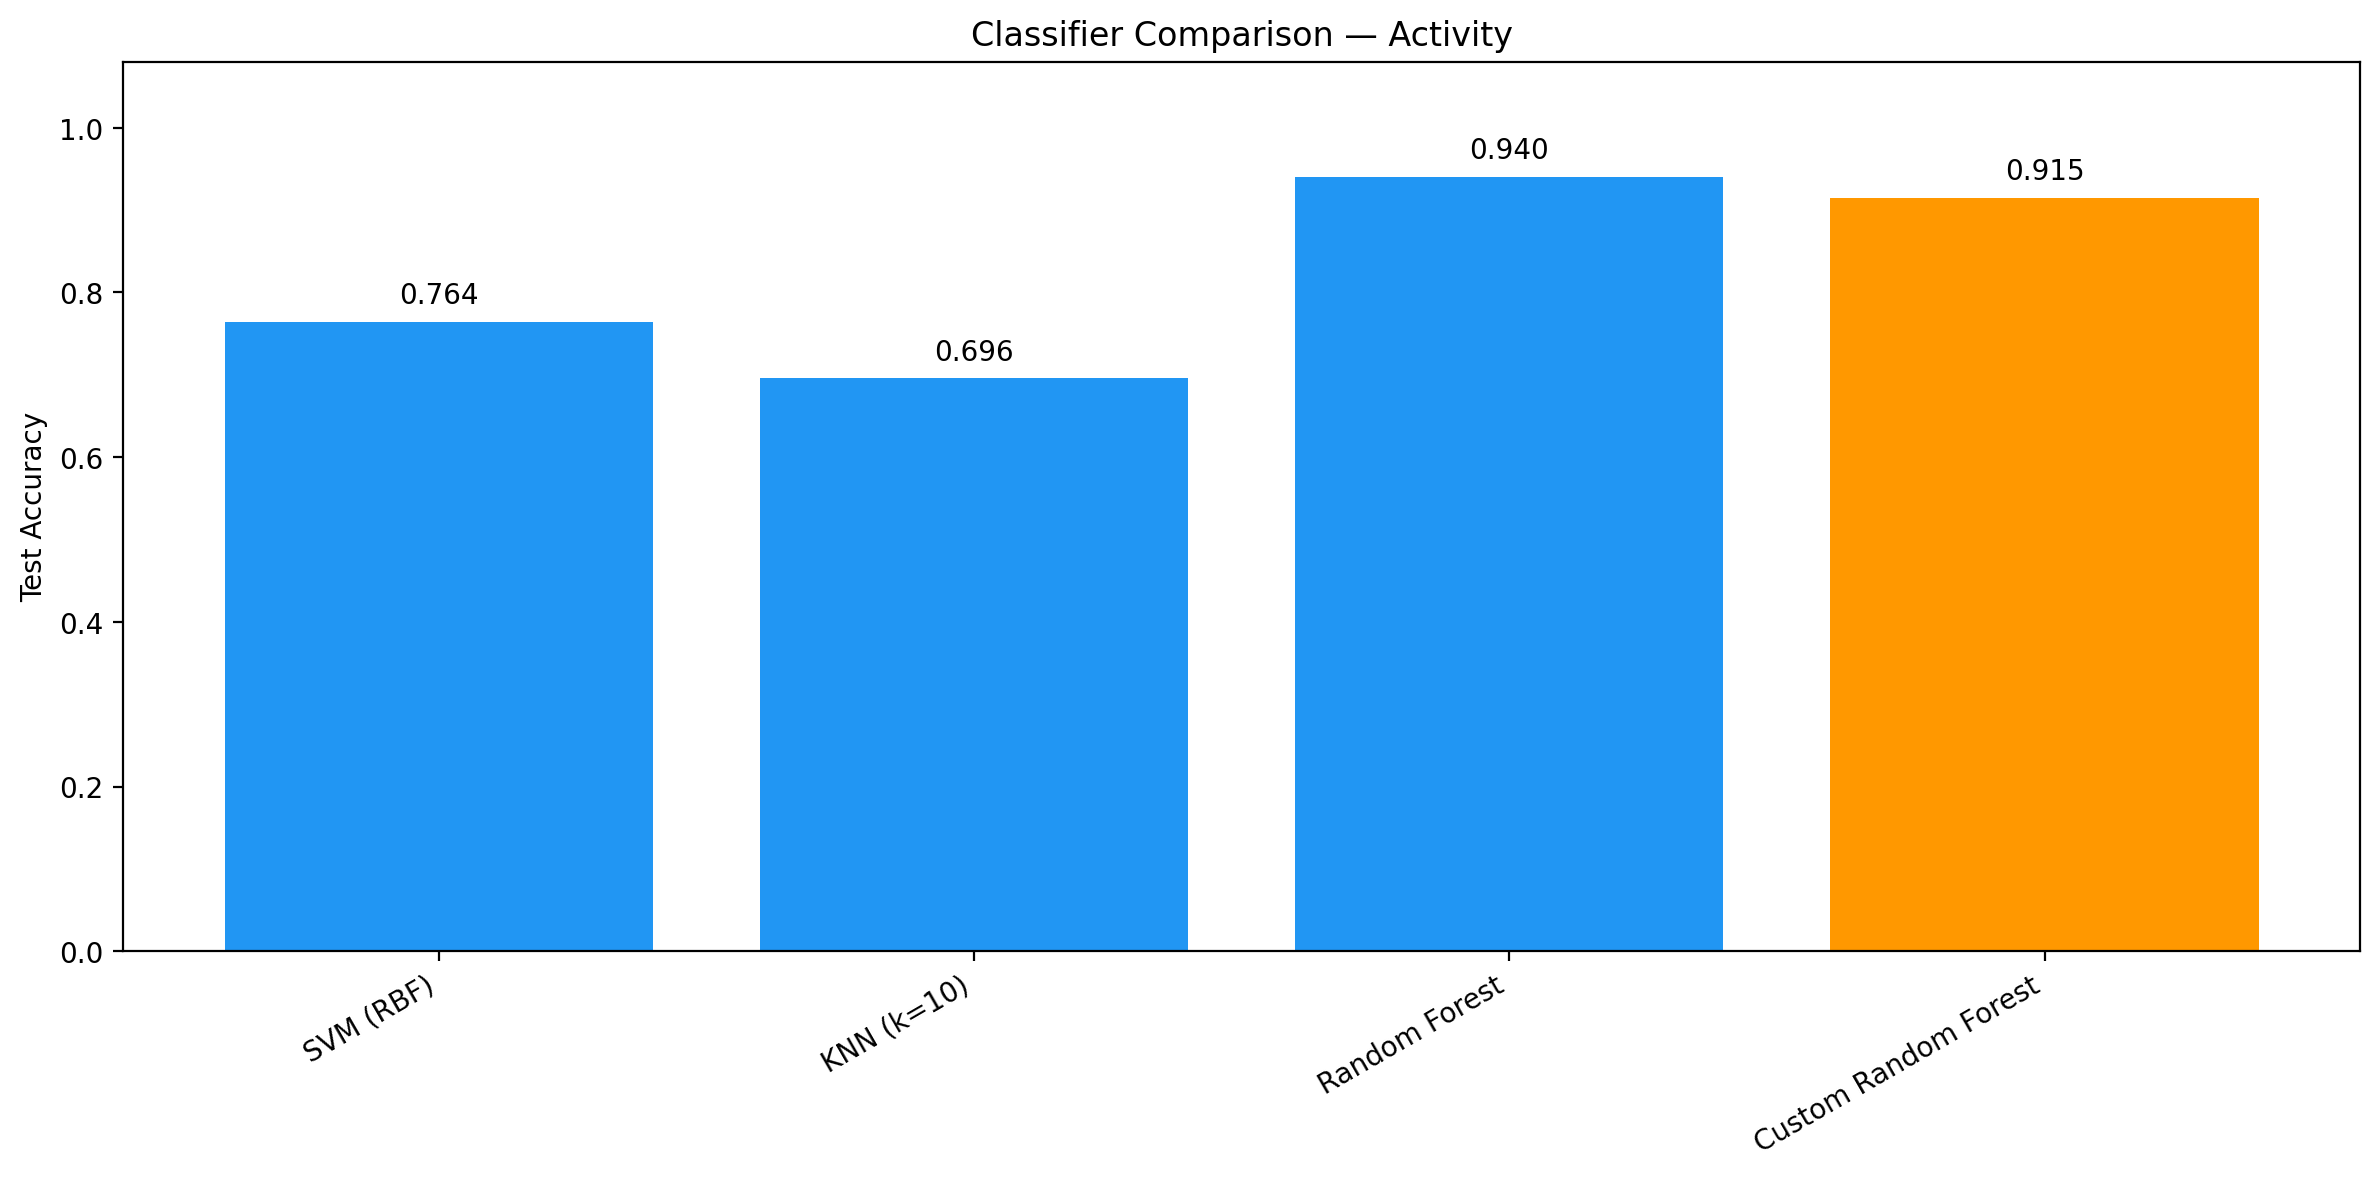
\includegraphics[width=0.7\textwidth]{img/accuracy_comparison_activity.png}
  
  \medskip
  \footnotesize Comparison of all four classifiers on activity detection.
\end{frame}

% Accuracy Comparison Distortion
\begin{frame}{Accuracy Comparison – Distortion Classification}
  \centering
  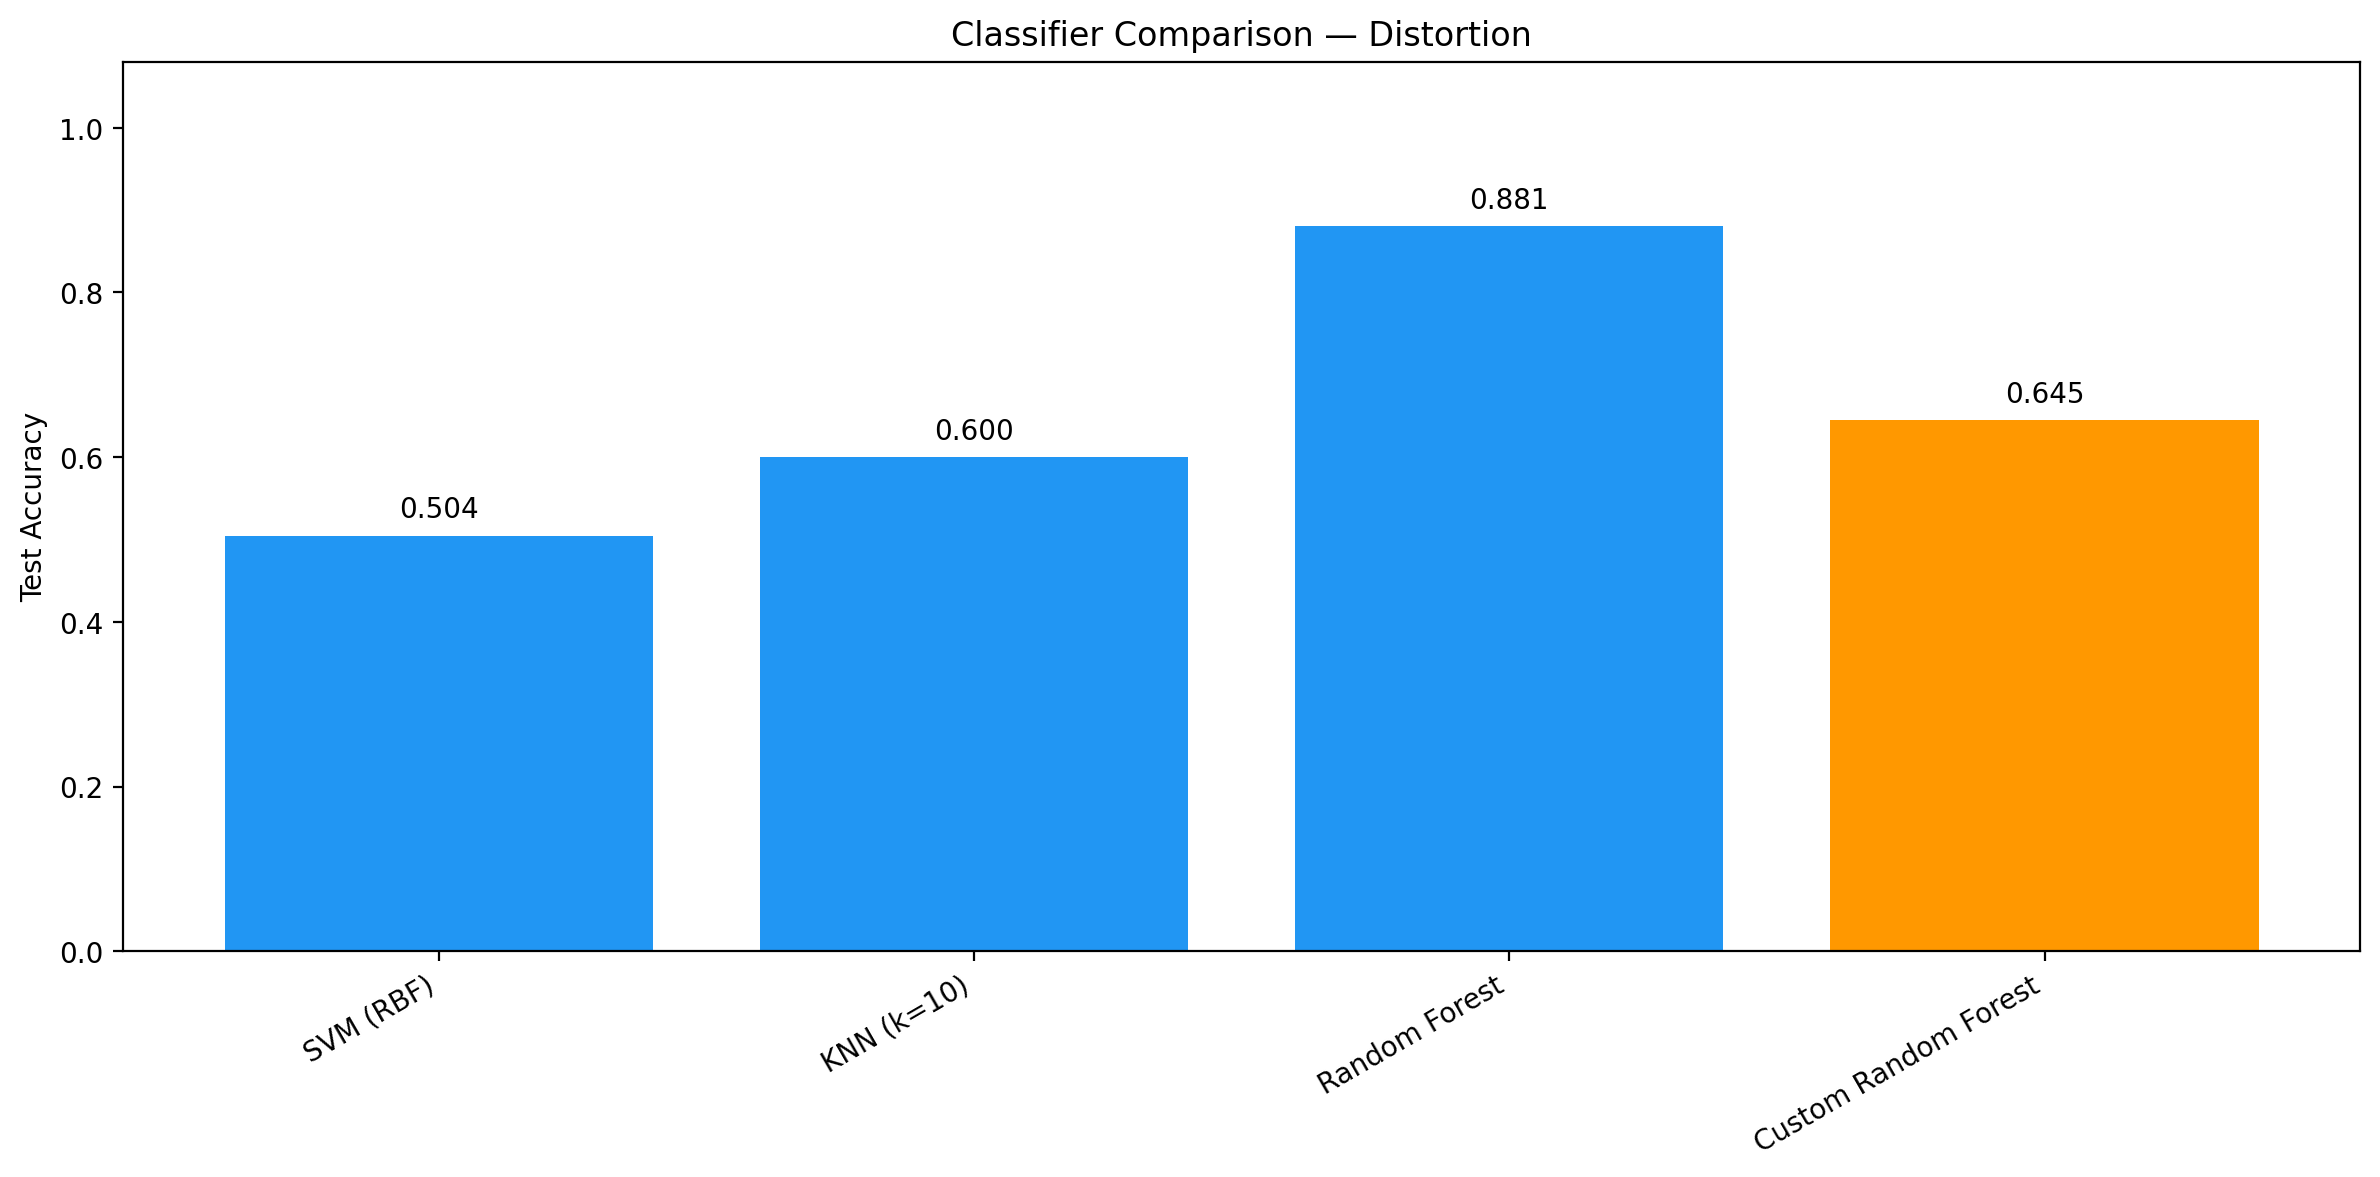
\includegraphics[width=0.7\textwidth]{img/accuracy_comparison_distortion.png}
  
  \medskip
  \footnotesize Comparison of all four classifiers on distortion type detection.
\end{frame}

% Custom RF Confusion Matrix
\begin{frame}{Custom Random Forest – Confusion Matrix}
  \centering
  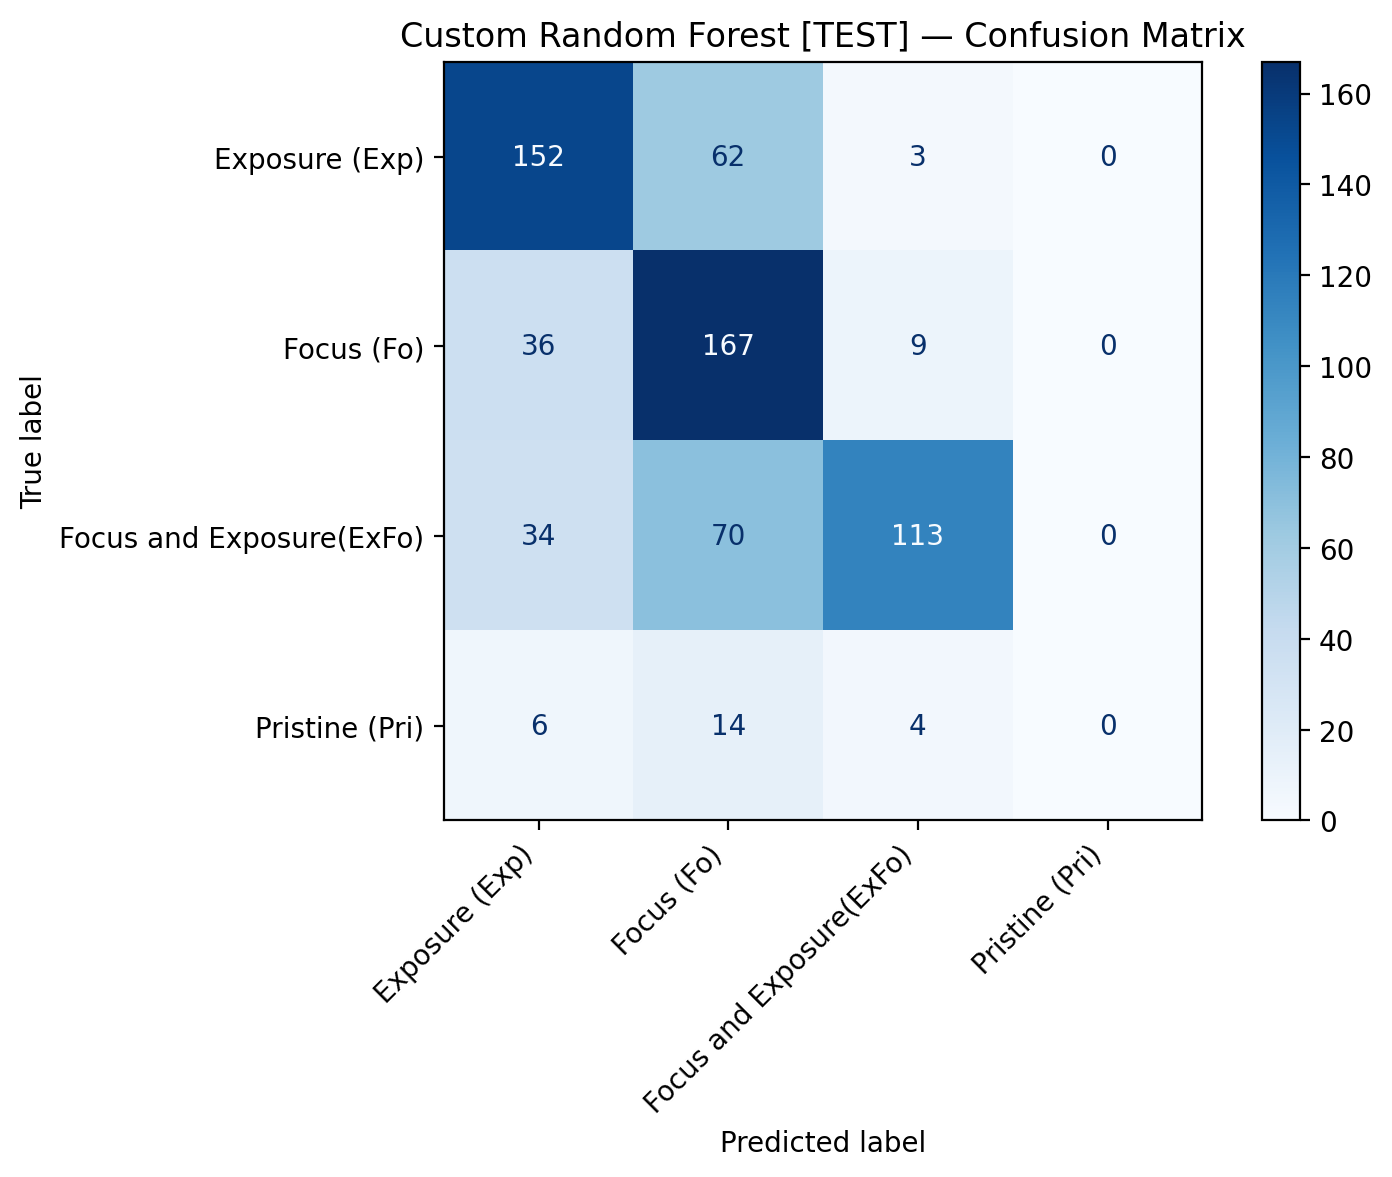
\includegraphics[width=0.7\textwidth]{img/cm_test_Custom_Random_Forest.png}
  
  \medskip
  \footnotesize Confusion matrix for Custom Random Forest implementation.
\end{frame}

\begin{frame}{Activity Classification – MOG2 Mode (848 videos)}
  \small
  \textbf{Severe class imbalance, only 128 test samples}
  \vspace{0.2cm}
  \begin{tabular}{lrr}
    \toprule
    Classifier & Test Acc. & CV Mean \\
    \midrule
    SVM (RBF)      & 62.5\% & 60.2\% \\
    KNN ($k=10$)   & 57.8\% & 55.9\% \\
    \alert{RF (sklearn)} & \alert{71.9\%} & 64.2\% \\
    Custom RF      & 68.4\% & 61.7\% \\
    \bottomrule
  \end{tabular}
  \vspace{0.3cm}
  \begin{itemize}
    \item Despite losing 81\% of videos to detection failures, motion features still carry discriminative signal.
    \item KNN suffers from 43‑dimensional feature space on small training set.
  \end{itemize}
\end{frame}

\begin{frame}{Distortion Classification – GT Mode (4 classes)}
  \small
  \textbf{Can we tell the distortion type from motion features alone?}
  \vspace{0.1cm}
  \begin{tabular}{lrr}
    \toprule
    Classifier & Test Acc. & CV Mean \\
    \midrule
    SVM (RBF)          & 50.4\% & 46.7\% \\
    KNN ($k=10$)       & 60.0\% & 55.9\% \\
    \alert{RF (sklearn)}  & \alert{88.1\%} & 84.6\% \\
    Custom RF          & 64.5\% & 61.9\% \\
    \midrule
    Random (4-class)   & 25.0\% & --- \\
    \bottomrule
  \end{tabular}
  \vspace{0.3cm}
  \begin{itemize}
    \item Distortion alters track stability, speed variance, and number of detected tracks.
    \item \textbf{First report of distortion classification accuracy on AD‑SVD.}
  \end{itemize}
\end{frame}

\begin{frame}{Detection – the Bottleneck}
  \centering
  \small
  \begin{tabular}{lll}
    \toprule
    Property & MOG2 (custom) & GT boxes \\
    \midrule
    Videos with tracks   & 848 (19\%)   & 4,461 (99.7\%) \\
    Class balance        & Severely imbalanced & Near‑balanced \\
    Best activity acc.   & 71.9\%       & \alert{94.0\%} \\
    \bottomrule
  \end{tabular}
  \vspace{0.4cm}
  \begin{itemize}
    \item \alert{81\% of videos filtered out} primarily by focus blur.
    \item The 26‑point accuracy gap is due to \textbf{detection failures}, not feature design.
    \item GT mode shows what the pipeline can achieve with \textbf{good detections}.
  \end{itemize}
\end{frame}

% ===========================================================================
\section{Conclusion}
% ===========================================================================

\begin{frame}{Key Findings}
  
  Beside the state of the art in activity classification :


  \begin{enumerate}
    \item Trajectory features (speed, straightness, spatial range) + simple Random Forest → \alert{94\% activity accuracy} under clean detections.
    \item Same features can classify the \alert{distortion type} with 88.1\% (4‑class), without pixel‑level quality inputs.
    \item The \alert{from‑scratch Random Forest} is only 1.5–3.5 pp behind the library version, quantifying the cost of hand‑rolling.
    \item Detection robustness is the \alert{main bottleneck}: MOG2 drops to 19\% of videos.
  \end{enumerate}
\end{frame}

\begin{frame}{Comparison with Deep Learning State‑of‑the‑Art}
  \small
  \begin{block}{Large‑scale action recognition benchmarks (Kinetics‑400, UCF101, HMDB51)}
    \begin{itemize}
      \item \textbf{I3D} (Carreira \& Zisserman, 2017) – inflated 3D ConvNets, top‑1 \(\sim 95\%\) (Kinetics). Needs massive labelled videos and GPU.
      \item \textbf{SlowFast} (Feichtenhofer et al., 2019) – two‑stream network for fine temporal resolution, state‑of‑the‑art accuracy but high compute.
      \item \textbf{VideoMAE} (Tong et al., 2022) – masked auto‑encoder with Vision Transformers, effective with limited data, but still GPU‑heavy.
      \item \textbf{Video Vision Transformer (ViViT)} (Arnab et al., 2021) – pure transformer model, strong but data‑hungry.
    \end{itemize}
  \end{block}
  \vspace{0.2cm}
  \begin{alertblock}{Our classical pipeline vs. deep learning}
    \begin{columns}[t]
      \column{0.48\textwidth}
      \textbf{Our Random Forest + hand‑crafted features}
      \begin{itemize}
        \item 94\% accuracy on 4,461 AD‑SVD videos (8 classes).
        \item Works on CPU, no GPU required.
        \item 43 interpretable motion features.
        \item Trained on only 3,100 videos.
      \end{itemize}
      \column{0.48\textwidth}
      \textbf{Typical deep learning approach}
      \begin{itemize}
        \item \(\geq 90\%\) on large‑scale benchmarks.
        \item Needs \(\sim\) millions of labelled videos.
        \item Requires GPU/TPU training.
        \item Black‑box features – hard to explain.
      \end{itemize}
    \end{columns}
  \end{alertblock}
  \vspace{0.1cm}
  \footnotesize
  Major citations: \alert{Carreira \& Zisserman, CVPR 2017}; \alert{Feichtenhofer et al., ICCV 2019}; \alert{Tong et al., NeurIPS 2022}; \alert{Arnab et al., ICCV 2021}.
\end{frame}

\begin{frame}{Limitations \& Future Work}
  \begin{block}{Limitations}
    \begin{itemize}
      \item MOG2 sensitive to lighting, shadows, and focus blur.
      \item Simple centroid tracker cannot handle occlusions or identity switches.
      \item Features omit intra-track dynamics (acceleration, periodicity).
    \end{itemize}
  \end{block}
  \vspace{0.2cm}
  \begin{exampleblock}{Future Work}
    \begin{itemize}
      \item Add acceleration statistics, FFT periodicity, and circular direction variance.
      \item Kalman‑filter or IoU‑based tracker for occlusion resilience.
      \item Distortion‑aware preprocessing (adaptive thresholding, deblurring).
      \item Real‑time stream classification with existing GUI.
    \end{itemize}
  \end{exampleblock}
\end{frame}

%----------------------------------------
%    CLOSING SLIDE
%----------------------------------------
\standout{\LARGE Thank You!\\\vspace{0.5cm}\Large Questions?}

\end{document}